\documentclass[UTF8, aspectratio=169, 9pt]{ctexbeamer}

\usepackage{graphicx}
\usepackage{booktabs}
\usepackage{color}
\usepackage{multirow}
\usepackage{fontspec}
\usepackage{amsmath}
\usepackage{amssymb}
\usepackage{tikz}
\usepackage{subfigure}
\usepackage{amsthm,amsfonts,mathtools}
%\usepackage[noend]{algpseudocode}
%\usepackage{algorithmicx,algorithm}
\usepackage[ruled]{algorithm2e}
\usepackage{textpos}
\usepackage{url}
\usepackage{algorithmic}

% \setmainfont{LMRomanUnsl10-Regular}
% \setmainfont{Noto Sans Mono CJK JP}
% \setmainfont{黑体}

% \useoutertheme{miniframes}
\usetheme{Goettingen}
% \usetheme{Madrid}
% \usetheme{Berkeley}
\title{组会汇报}
\subtitle{基于Game Theory的交互决策}
\author{李鑫}
\institute{吉林大学}
\date{\today}
\begin{document}
\frame{\titlepage}
\frame{\tableofcontents}


\section{背景}
\subsection{自动驾驶中的决策/规划问题}
\begin{frame}
 \frametitle{示意问题}
\begin{figure}[htbp]
\centering

\subfigure[从A到B问题.]{
\begin{minipage}[t]{0.5\linewidth}
\centering
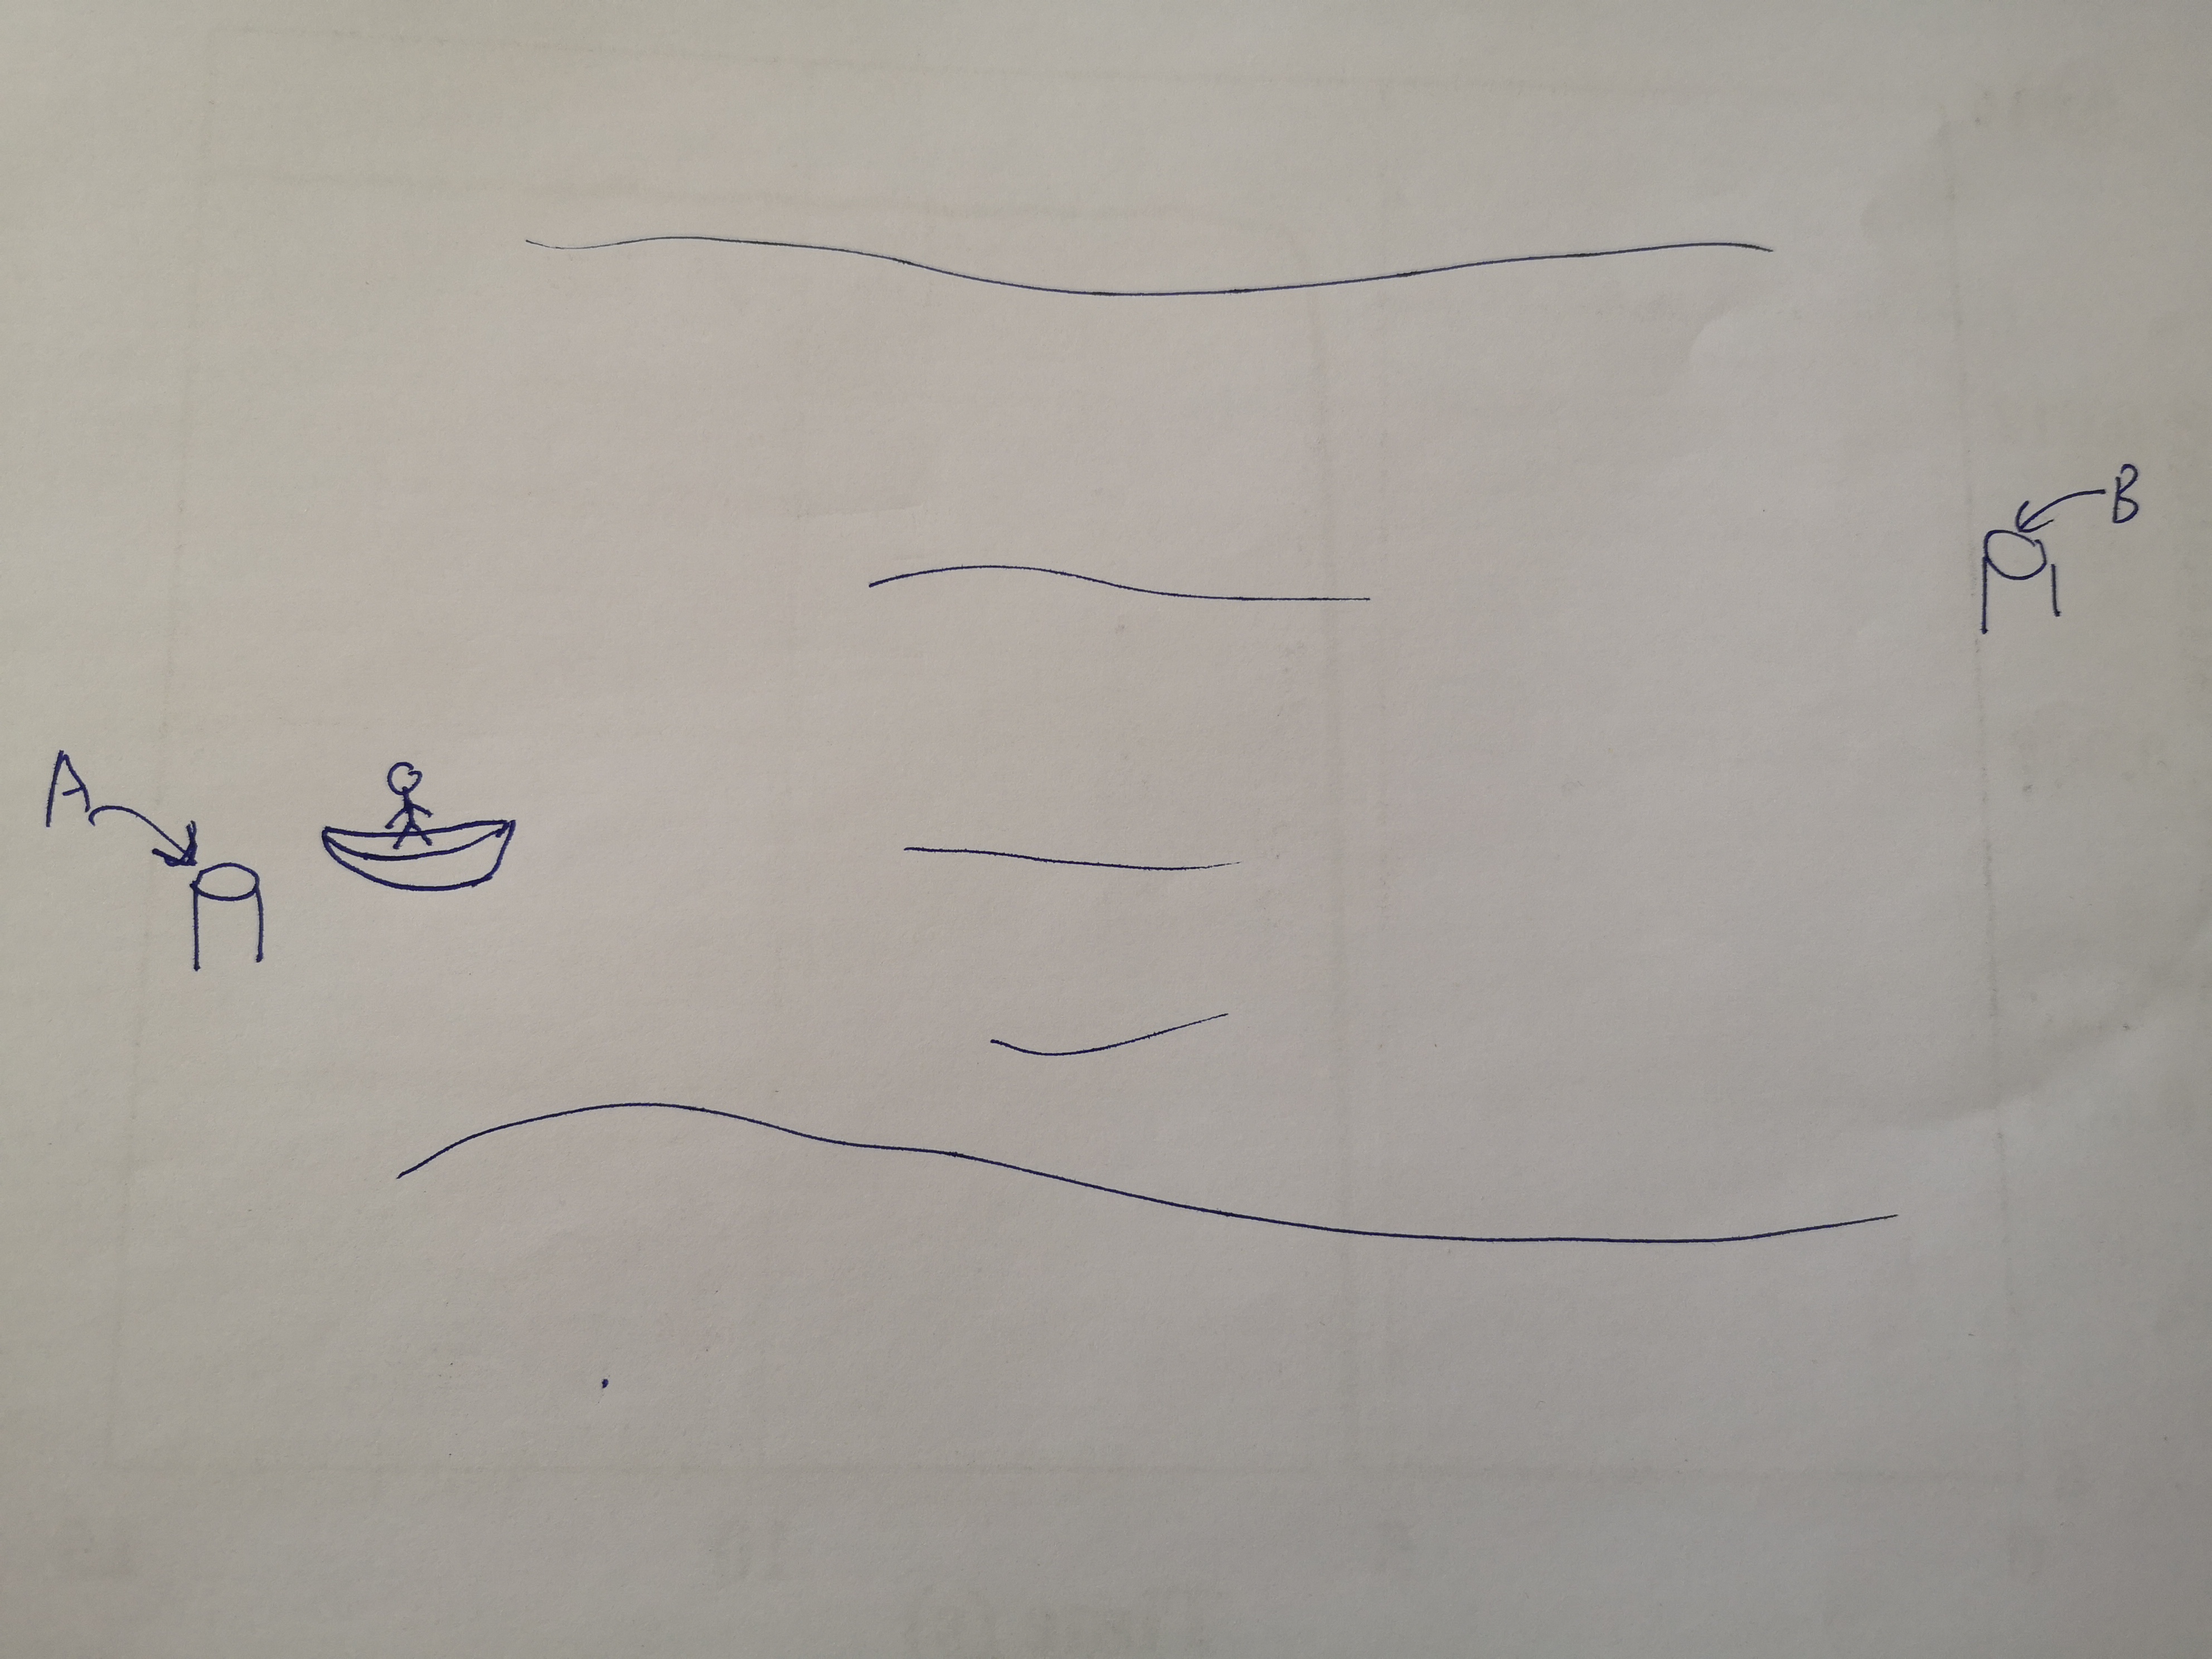
\includegraphics[height=1in,width=2in]{1.jpg}
%\caption{fig1}
\end{minipage}%
}%
\subfigure[从A到B,有静态障碍物的问题.]{
\begin{minipage}[t]{0.5\linewidth}
\centering
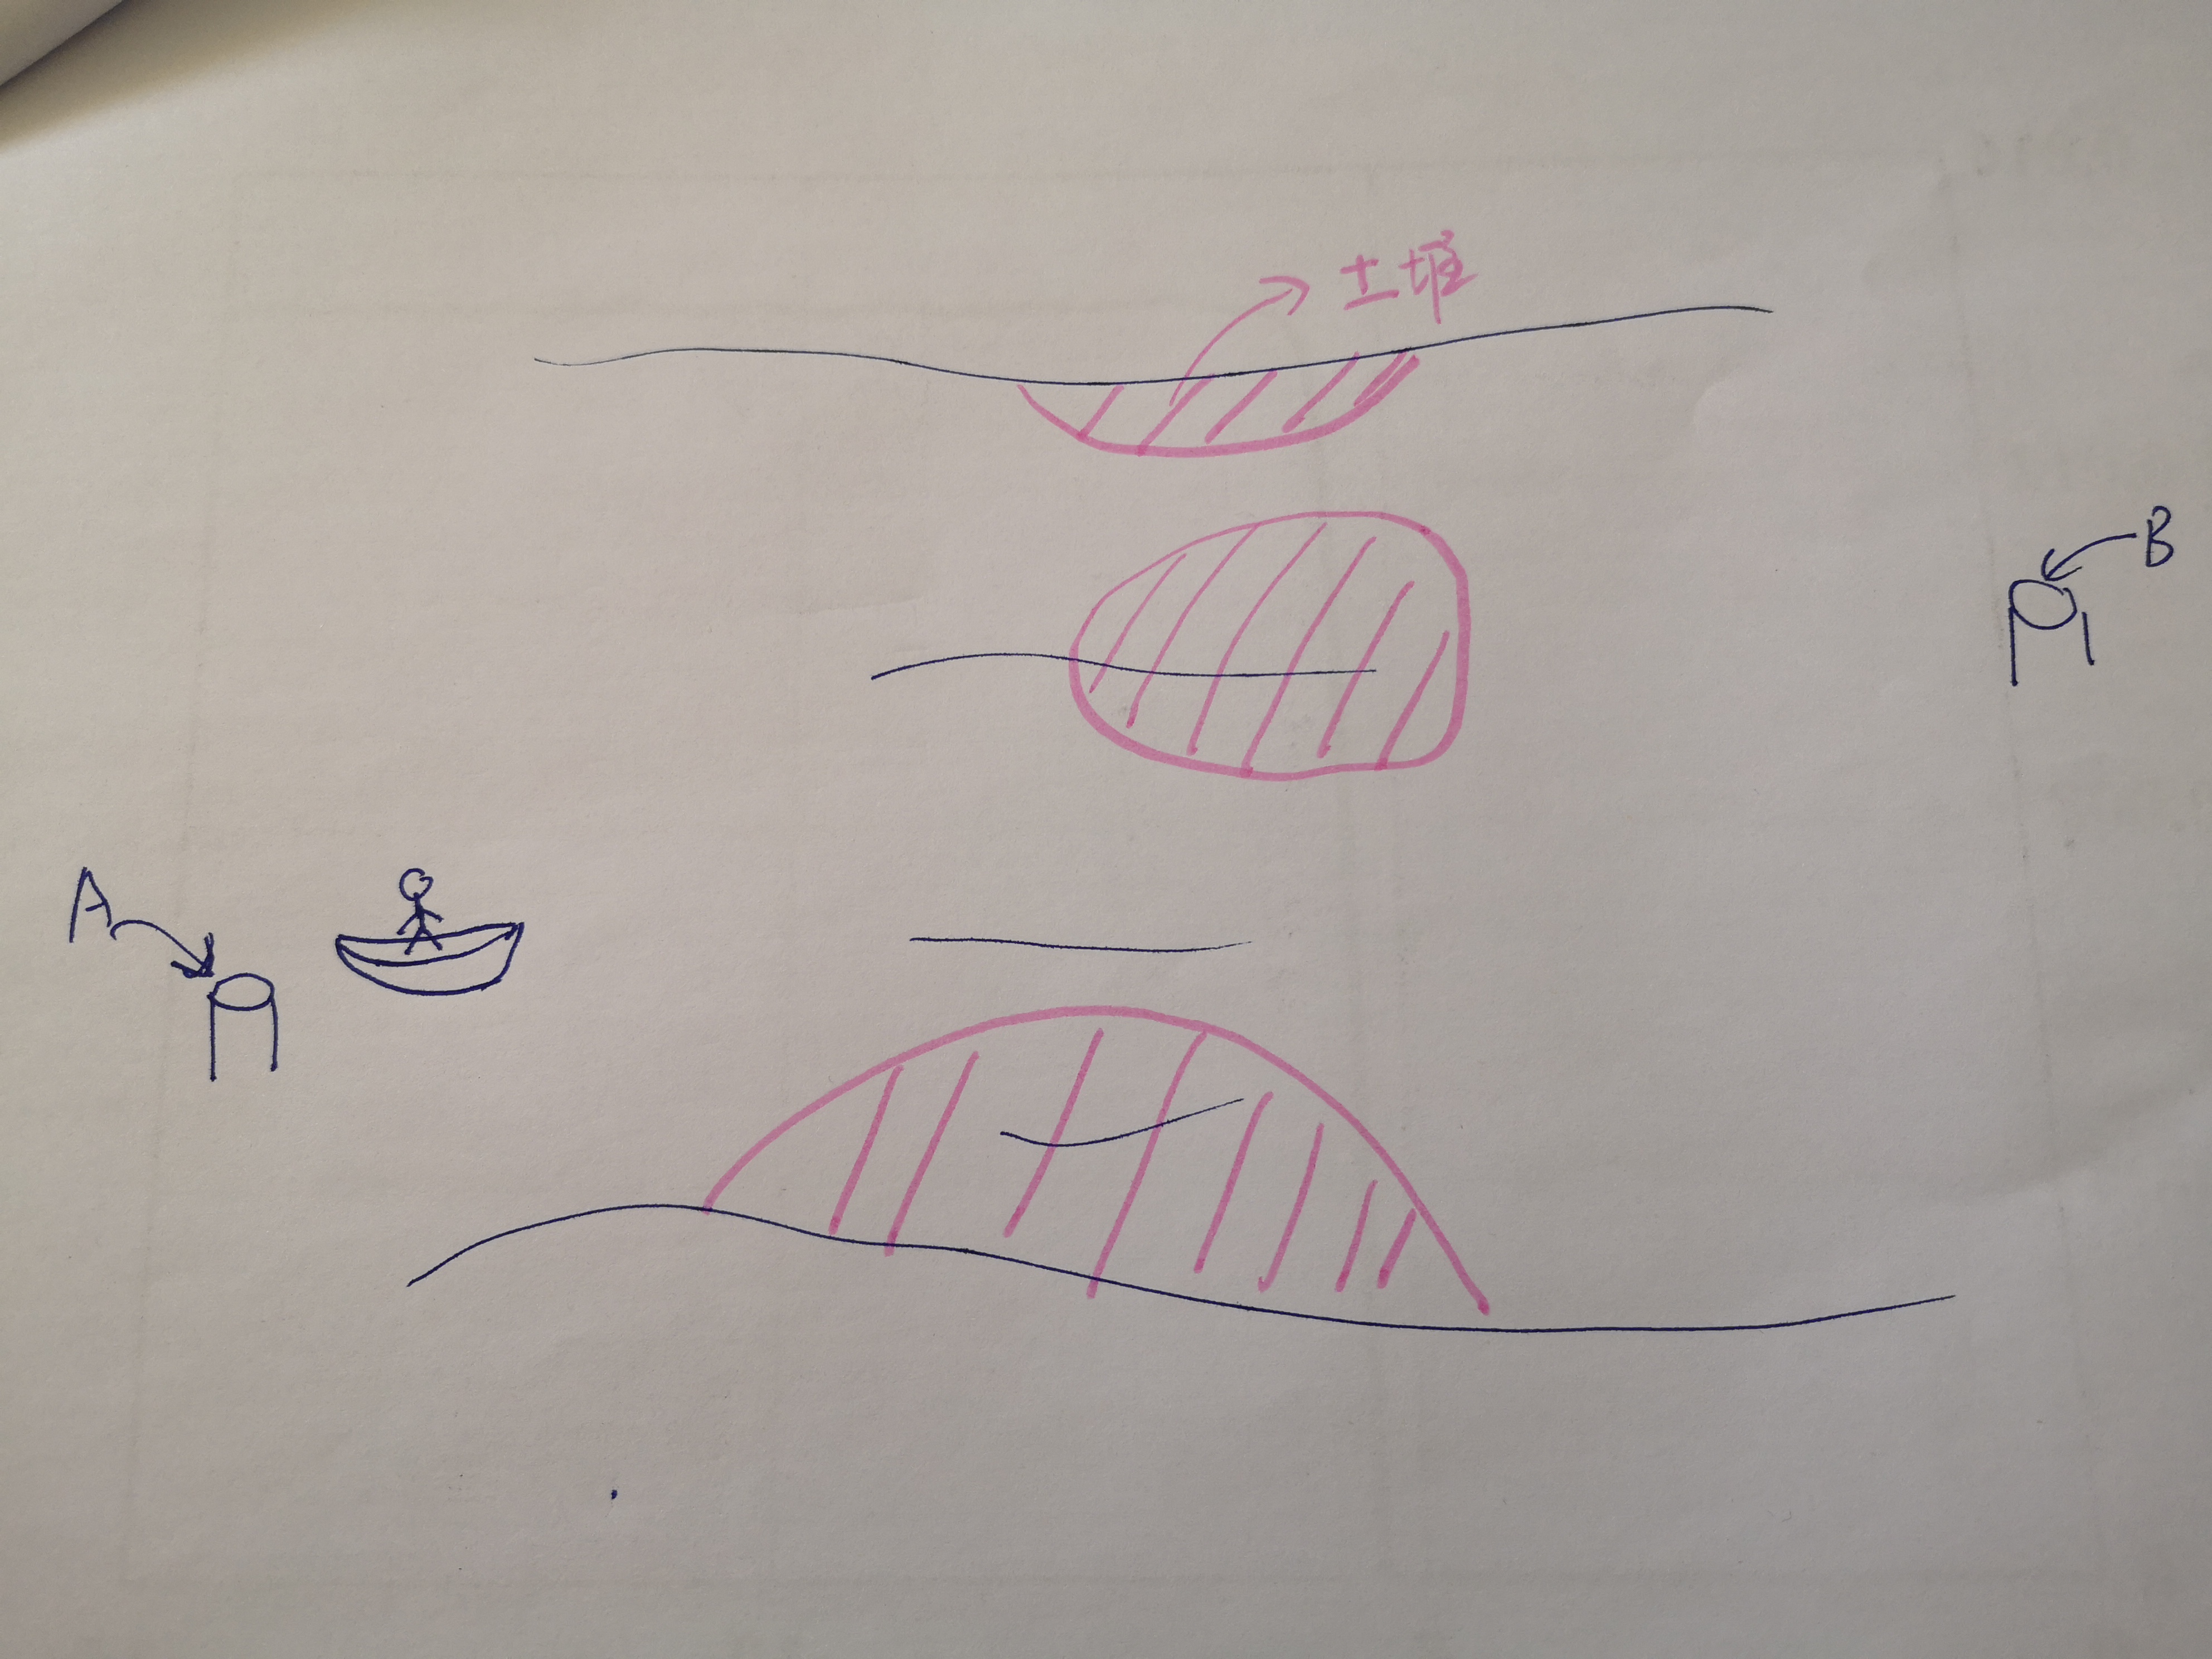
\includegraphics[height=1in,width=2in]{2.jpg}
%\caption{fig2}
\end{minipage}%
}%

%这个回车键很重要 \quad也可以
\subfigure[从A到B,有动态障碍物的问题.]{
\begin{minipage}[t]{0.5\linewidth}
\centering
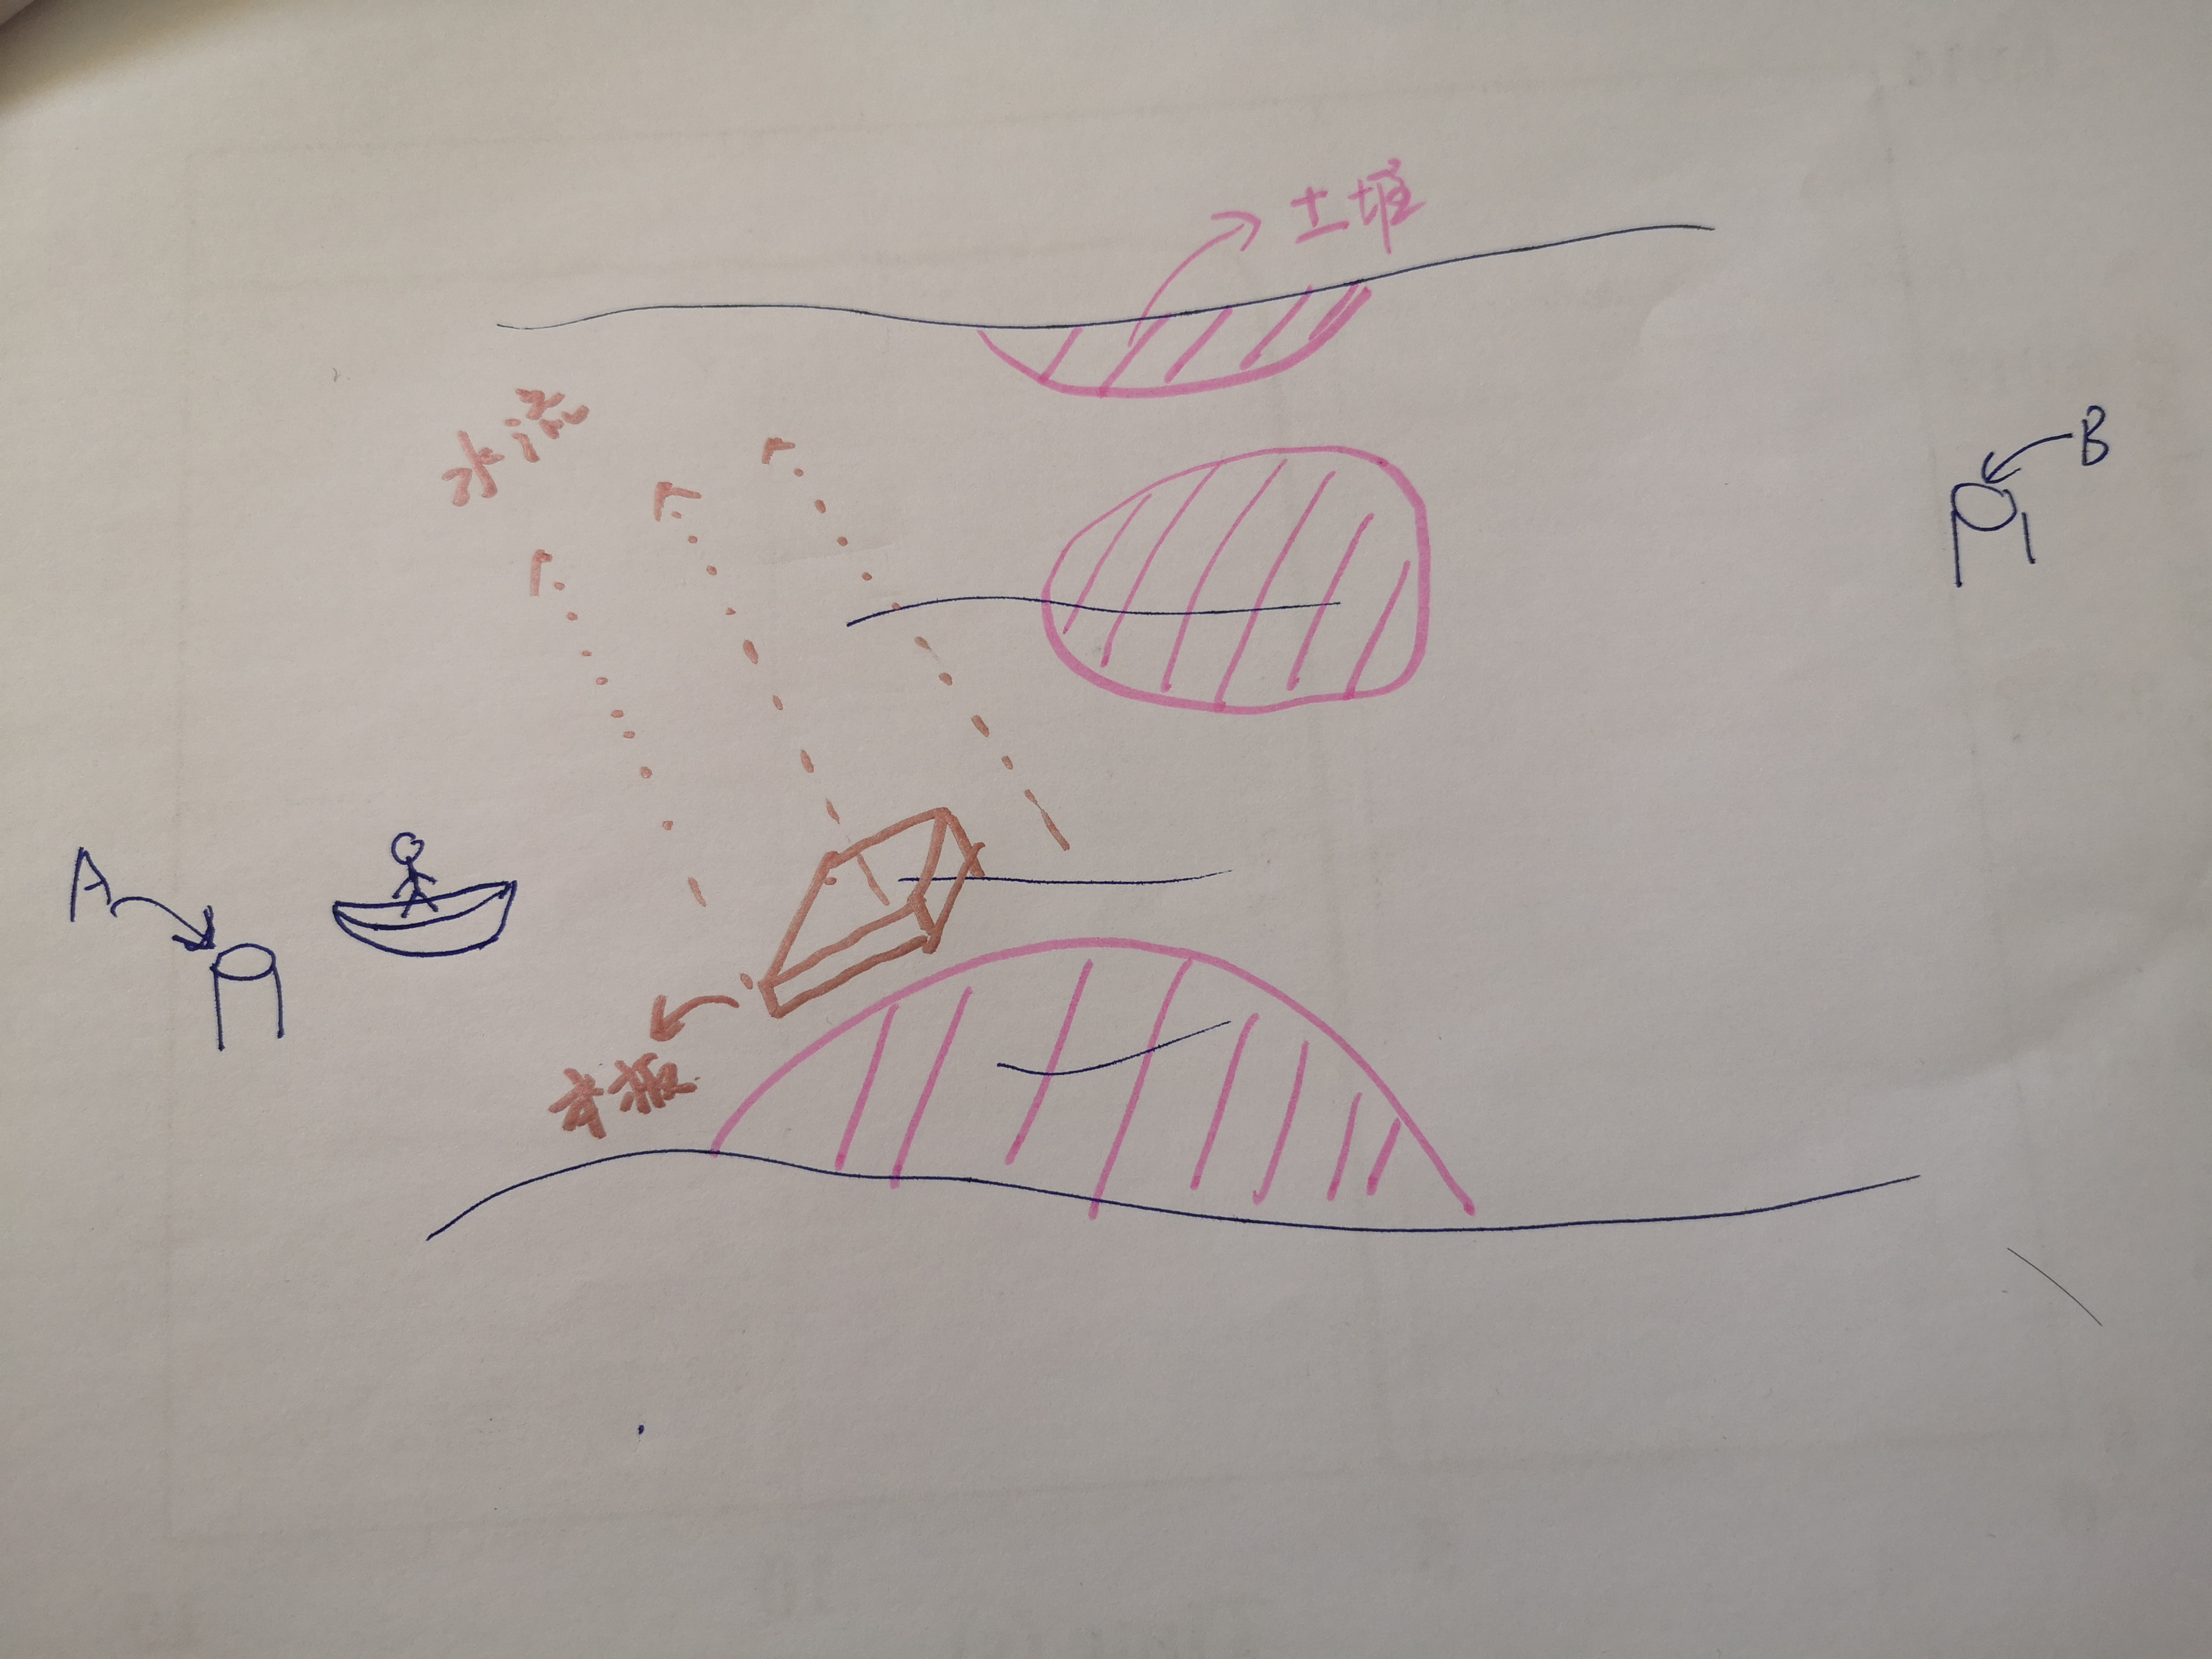
\includegraphics[height=1in,width=2in]{3.jpg}
%\caption{fig2}
\end{minipage}
}%
\subfigure[从A到B,有动态智能体的问题.]{
\begin{minipage}[t]{0.5\linewidth}
\centering
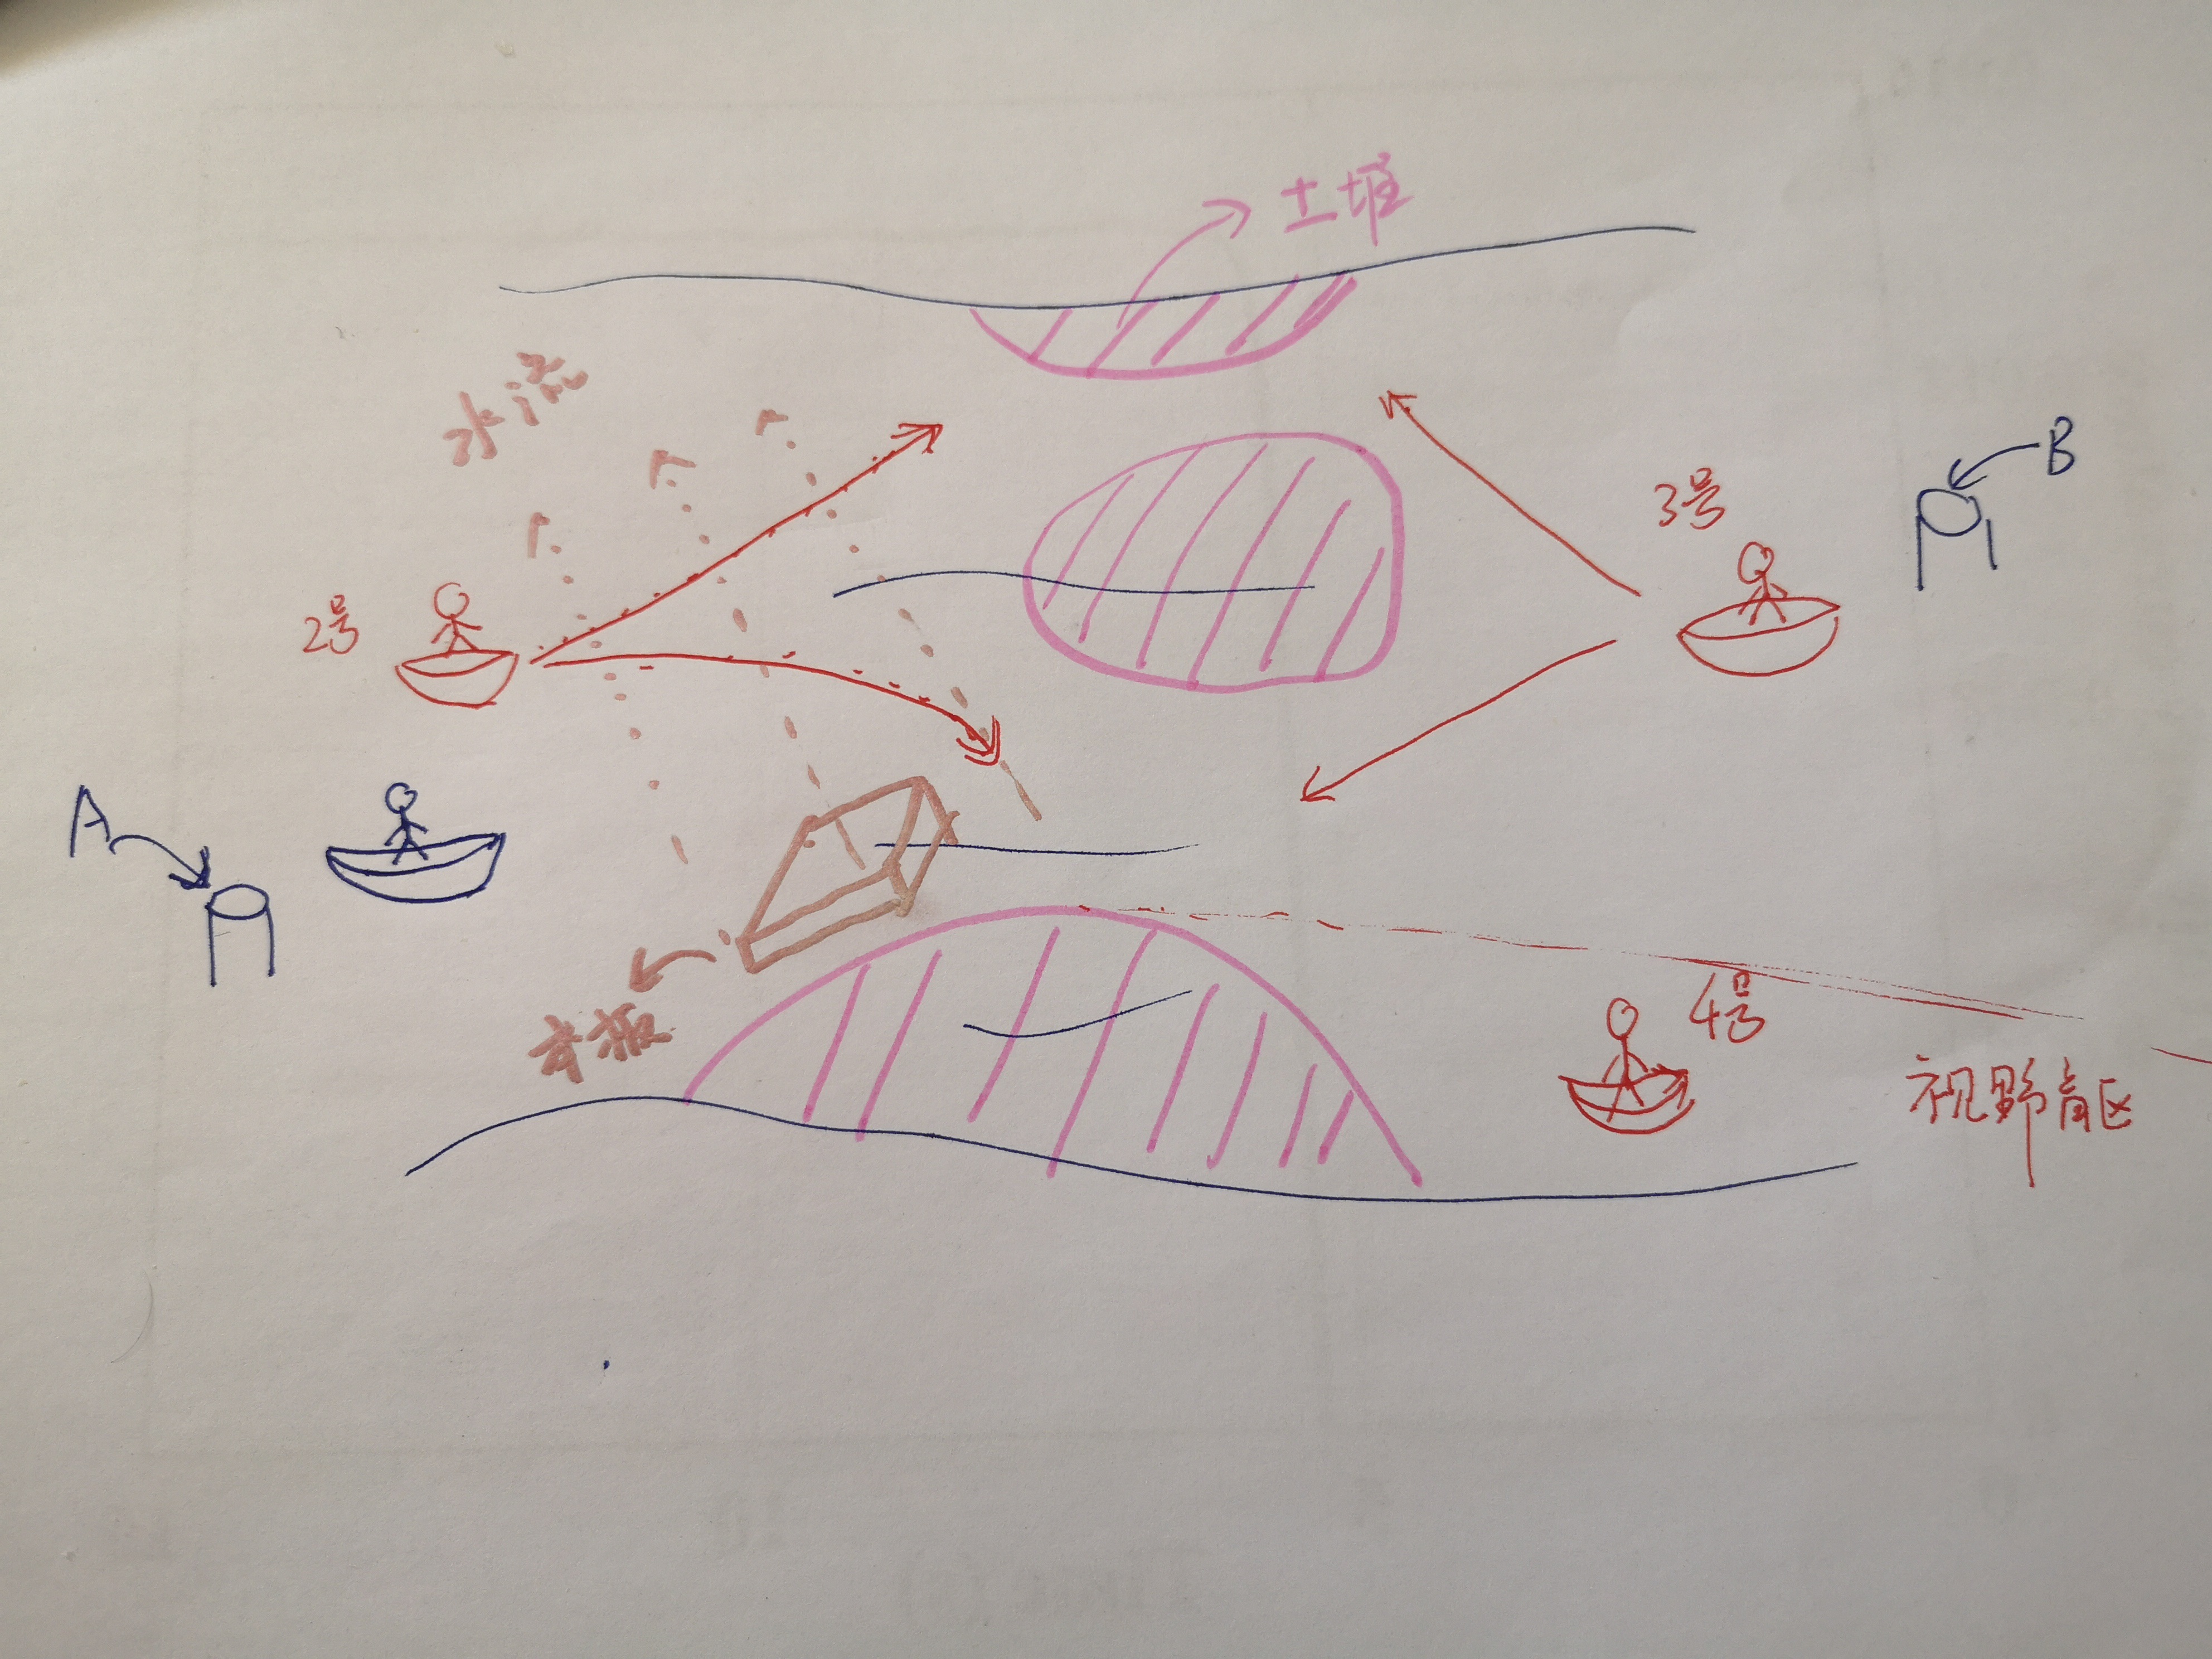
\includegraphics[height=1in,width=2in]{4.jpg}
%\caption{fig2}
\end{minipage}
}%

%\centering
%\caption{ pics}
\end{figure}
\end{frame}

\subsection{最优控制回顾}
\subsubsection{经典变分}
\begin{frame}
  \frametitle{变分法回顾}
  \begin{itemize}
  \item 寻找$f(x)$的局部极小点的必要条件($x_{\min}$)
    \begin{align*}
      \frac{dy}{dx} = 0
    \end{align*}.
  \item 只能得到驻点/临界点(stationary/critial points),需要进一步验证.
  \item 对于泛函($I[f]$),可以通过类似方法得到Stationary functions of a functional.
  \item 一般而言, 通过需找一个函数 $y=f(x)$ 使得下面的积分:
    \begin{align*}
      I[f] = \int_{x_1}^{x_2} F( x, y, \frac{dy}{dx} ) dx
    \end{align*}
    stationary.
  \end{itemize}
\end{frame}

\begin{frame}
  \frametitle{Euler-Lagrange 方程推导}
  \begin{itemize}
  \item 假设 $y(x)$ 使得泛函 $I[f]$ stationary 且满足边值条件 $y(x_1) = y_1, \, y(x_2) = y_2$.
  \item 引入辅助函数 $\eta, 满足 \eta (x_1) = \eta (x_2) = 0$.
  \item 构造一个函数 $\bar{y} = \textcolor{red} {y(x)} + \epsilon \eta(x)$ 可以容易得到这个函数和$y(x)$一样满足边值条件,这样构造出来的函数可以表示满足边值条件的函数族.
  \item 在这一族函数里面找特定的函数 $\bar{y} (x)$ 满足泛函stationary的条件,因为构造出来的函数可以通过改变$\epsilon$来改变,所以泛函可以表示为 $I( \epsilon ) =
    \int_{x_1}^{x_2} F( x, \bar{y}, \bar{y}' )$ .
  \item 这样构造出来的泛函只和$\epsilon$有关,变成了一维问题, 所以一阶条件变成了
    $\frac{dI}{d \epsilon} |_{\epsilon = 0} = 0$,

    \begin{align}
      \begin{split}
        & \frac{d}{d \epsilon} |_{\epsilon = 0} \, \int_{x_1}^{x_2} F(x,
        \bar{y}, \bar{y}' ) dx = 0 \Rightarrow \int_{x_1}^{x_2}
        \frac{\partial}{\partial
          \epsilon} F( x, \bar{y}, \bar{y}' ) |_{\epsilon} dx = 0 \\
        \Rightarrow & \int_{x_1}^{x_2} \big [ \frac{ \partial F }{ \partial
          \bar{y} } \frac{ \partial \bar{y} }{ \partial \epsilon } + \frac{
          \partial F }{ \partial \bar{y}' } \frac{ \partial \bar{y}' }{ \partial
          \epsilon } \big ] |_{\epsilon=0} dx = 0
        \Rightarrow  \int_{x_1}^{x_2} \big [ \frac{ \partial F }{ \partial
          \bar{y} } \eta (x) + \frac{
          \partial F }{ \partial \bar{y}' } \textcolor {blue} {\eta'(x)} \big ] |_{\epsilon=0} dx =
        0 \\
        \Rightarrow & \int_{x_1}^{x_2} \big [ \frac{ \partial F }{ \partial
          \bar{y} } \eta (x) - \frac{d}{dx} \big ( \frac{
          \partial F }{ \partial \bar{y}' } \big ) \eta(x) \big ] |_{\epsilon=0} dx =
        0
        \Rightarrow  \int_{x_1}^{x_2} \big [ \frac{ \partial F }{ \partial
          \bar{y} }  - \frac{d}{dx} \big ( \frac{
          \partial F }{ \partial \bar{y}' } \big )  \big ] \eta(x) |_{\textcolor
          {red} {\epsilon=0} } dx =
        0  \\
        \Rightarrow & \int_{x_1}^{x_2} \big [ \frac{ \partial F }{ \partial
          \textcolor {red} {y} }  - \frac{d}{dx} \big ( \frac{
          \partial F }{ \partial \textcolor {red} {y} } \big )  \big ] \eta(x)  dx =
        0
        \Rightarrow \textcolor[rgb]{1.00,0.00,0.00}{ \frac{ \partial F }{ \partial
          {y} }  - \frac{d}{dx} \big ( \frac{
          \partial F }{ \partial  {y} } \big )  = 0 }
      \end{split}
    \end{align}.

  \end{itemize}
\end{frame}

\subsubsection{PMP必要条件}
\begin{frame}
  \frametitle{庞特里亚金极大值原理回顾}
  \begin{itemize}
    \item 一般优化控制问题
    \begin{align}
      \begin{split}
\max  \, & \int_{0}^{T} L(t, x(t), u(t)) \mathrm{d} t+\Psi(T, x(T)) \\
 \text { s.t. } & \dot{x}(t)=f(t, x(t), u(t)), \quad \text { a.e. } t \in[0, T] \\
& x(0)=x_{0} \\
& (T, x(T)) \in \mathcal{T} \subseteq \mathbb{R}^{n+1} \\
& u(t) \in U \subseteq \mathbb{R}^{m}, \quad \text { a.e. } t \in[0, T]
\end{split}
    \end{align}
    \item Bolza form
    $$ \int_{0}^{T} L(t, x(t), u(t)) \mathrm{d} t+\Psi(T, x(T)) $$
    \item Lagrange form
    $$ \int_{0}^{T} L(t, x(t), u(t)) \mathrm{d} t
    $$
    \item Mayer form
    $$ \Psi(T, x(T))
    $$
  \end{itemize}
\end{frame}

\begin{frame}
\frametitle{没有终端约束的PMP推导 }
拉格朗日形式
$$
  \mathcal{L}(x, u, p):=\Psi(x(T))+\int_{0}^{T} p(t)(f(t, x(t), u(t))-\dot{x}(t)) \mathrm{d} t,
$$
对$x$求偏导
$$
D_{x} \mathcal{L}(x, u, p) z=\nabla \Psi(x(T)) z(T)+\int_{0}^{T} p(t)\left(D_{x} f(t, x(t), u(t)) z(t)-\dot{z}(t)\right) \mathrm{d} t
$$
分部积分得到
\begin{align*}
  \begin{split}
  D_{x} \mathcal{L}(x, u, p) z=&(\underbrace{\nabla \Psi(x(T))-p(T)}_{\text {终端条件 } p}) z(T)+p(0) \underbrace{z_{0}}_{=0} \\
&+\int_{0}^{T}(\underbrace{p(t) D_{x} f(t, x(t), u(t))+\dot{p}(t)}_{\text {动态条件 } p}) z(t) \mathrm{d} t
  \end{split}
\end{align*}
\end{frame}



\begin{frame}
\frametitle{没有终端约束的PMP推导 }
\begin{theorem}
  设$u^*$ 是最优控制,$x^*$是相应的状态轨迹,$p:[0,T] \rightarrow \mathbb{R}^{n,*}$是adjoint equation的解
  $$
  \dot{p}(t)=-p(t) D_{x} f\left(t, x^{*}(t), u^{*}(t)\right),
  $$
  同时满足
  $$
  p(T)=\nabla \Psi\left(x^{*}(T)\right).
  $$
  则,PMP最大值原理条件为
  $$
  p(t) f\left(t, x^{*}(t), u^{*}(t)\right)=\max _{\omega \in U} p(t) f\left(t, x^{*}(t), \omega\right), \quad \text { a.e. } \quad t \in[0, T]
  $$
\end{theorem}
定义 Hamiltonian 为$H(t, x, u, p):=p f(t, x, u)$,那么PMP就是在说满足
$
\dot{p}(t)=-D_{x} H\left(t, x^{*}(t), u^{*}(t), p(t)\right), \quad p(T)=\nabla \Psi\left(x^{*}(T)\right)
$
最大值条件为
$$H\left(t, x^{*}(t), u^{*}(t), p(t)\right)=\max _{\omega \in U} H\left(t, x^{*}(t), \omega, p(t)\right), \quad \text { a.e. } \quad t \in[0, T]
$$
\end{frame}

\begin{frame}
\frametitle{证明 }

  在$L1$意义下局部最优:存在$\epsilon > 0$使得在$\| u - u^* \|_1$可行域$(x,u)$内存在最优局部解为$(x^*, u^*)$.
  对于$\{ (x_{\epsilon}, u_{\epsilon}) \}_{\epsilon > 0 }$ 一族轨迹控制对, 假设$u_{\epsilon}$在$L1$意义下$\epsilon \rightarrow 0_+$ 趋近与$u^*$, 则我们可以得到
  \begin{align*}
  \begin{split}
  0 \ge \frac{\partial}{\partial \epsilon} \bigg |_{\epsilon=0_+} \Psi( x_{\epsilon}(T) ) & = \lim_{\epsilon \to 0_+} \frac{\Psi(x_{\epsilon}(T)) - \Psi( x^*(T) )}{\epsilon} \\
   &= \nabla \Psi(x^*(T)) \frac{\partial}{\partial \epsilon} \bigg |_{\epsilon=0_+} x_{\epsilon}(T) = p(T) \frac{\partial}{\partial \epsilon} \bigg |_{\epsilon=0_+} x_{\epsilon}(T)
  \end{split}
  \end{align*}

  但是我们想要得到的是
  $$
  0 \geq p(\tau)\left(f\left(\tau, x^{*}(\tau), \omega\right)-f\left(\tau, x^{*}(\tau), u^{*}(\tau)\right)\right), \text { a.e. on }[0, T], \quad \text { for all } \omega \in U
  $$

  下面从局部最优条件推导出结论需要两个工具
  \begin{itemize}
    \item The adjoint and the variational equations:
    推导出符号一致性
    \item Perturbations of optimal control: needle variations:
    推导出最优性
  \end{itemize}


\end{frame}

\begin{frame}
\frametitle{证明(继续) }

(1)对于$y \in \mathbb{R}^n$,$v:[\tau, T] \to \mathbb{R}^m$是PDE
$$
\dot{v}(t)=D_{x} f\left(t, x^{*}(t), u^{*}(t)\right) v(t), \qquad v(\tau)=\mathrm{y}
$$
的解,构造$x_{\varepsilon}(\tau)=x^{*}(\tau)+\varepsilon \mathbf{y}+o(\varepsilon)$.那么对于所有$t \ge \tau , $
$$
v(t)=\left.\frac{\partial}{\partial \varepsilon}\right|_{\varepsilon=0^{+}} x_{\varepsilon}(t)
$$

\begin{figure}
  \centering
  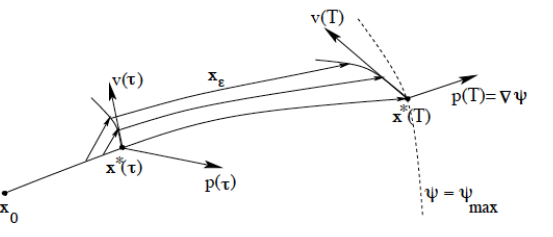
\includegraphics[width=8cm]{variationalequation.png}
  \caption{from Bressan-Piccolo's book}
\end{figure}
\end{frame}

\begin{frame}
\frametitle{证明(继续) }
对于这样的方程
$$
\left\{\begin{array}{l}
\dot{v}(t)=D_{x} f\left(t, x^{*}(t), u^{*}(t)\right) v(t) \\
\dot{p}(t)=-p(t) D_{x} f\left(t, x^{*}(t), u^{*}(t)\right)
\end{array}\right.
$$
我们可以得到
$$
t \mapsto p(t) \cdot v(t) \text { is constant. }
$$
目前为止我们得到的条件有
$$
0 \geq\left. p(T) \frac{\partial}{\partial \varepsilon}\right|_{\varepsilon=0^{+}} x_{\varepsilon}(T)
\Rightarrow
0 \geq\left. p(\tau) \frac{\partial}{\partial \varepsilon}\right|_{\varepsilon=0^{+}} x_{\varepsilon}(\tau)
$$
我们想证明是
$$
0 \geq p(\tau)\left(f\left(\tau, x^{*}(\tau), \omega\right)-f\left(\tau, x^{*}(\tau), u^{*}(\tau)\right)\right)
$$
那么现在只要证明
$$
\left.\frac{\partial}{\partial \varepsilon}\right|_{\varepsilon=0^{+}} x_{\varepsilon}(\tau)=\underbrace{f\left(\tau, x^{*}(\tau), \omega\right)-f\left(\tau, x^{*}(\tau), u^{*}(\tau)\right)}_{\mathrm{y}}.
$$
\end{frame}

\begin{frame}
\frametitle{证明(继续) }
定义needle variations, 对于$\tau \in (0,T], \omega \in U, 0 < \epsilon < \tau$
$$
u_{\varepsilon}(t):=\left\{\begin{array}{cl}
\omega, & \text { if } t \in[\tau-\varepsilon, \tau] \\
u^{*}(t), & \text { if not. }
\end{array}\right.
$$
\begin{figure}
  \centering
  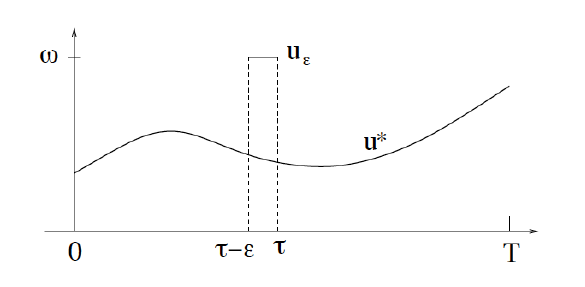
\includegraphics[width=8cm]{needle.png}
\end{figure}

我们宣称(Claim):
$$
\left.\frac{\partial}{\partial \varepsilon}\right|_{\varepsilon=0^{+}} x_{\varepsilon}(\tau)=f\left(\tau, x^{*}(\tau), \omega\right)-f\left(\tau, x^{*}(\tau), u^{*}(\tau)\right), \quad \text { for a.e. } \tau \in(0, T].
$$
\end{frame}

\begin{frame}
\begin{proof}[证明(最后一页)]
  由定义可知
  $$
  \frac{x_{\varepsilon}(\tau)-x^{*}(\tau)}{\varepsilon}=\frac{1}{\varepsilon}\left\{\int_{\tau-\varepsilon}^{\tau} f\left(t, x_{\varepsilon}(t), \omega\right) \mathrm{d} t-\int_{\tau-\varepsilon}^{\tau} f\left(t, x^{*}(t), u^{*}(t)\right) \mathrm{d} t\right\}
  $$
  很容易可以观察到后面一项:
  $$
  \frac{1}{\varepsilon} \int_{\tau-\varepsilon}^{\tau} f\left(t, x^{*}(t), u^{*}(t)\right) \mathrm{d} t \underset{\varepsilon \rightarrow 0^{+}}{\longrightarrow} f\left(\tau, x^{*}(\tau), u^{*}(\tau)\right)
  $$
  如果$\tau$是$t \mapsto f(t, x^*(t),u^*(t))$的Lebesgue point那么我们可以得到:

  \begin{align*}
    \begin{split}
        \frac{1}{\varepsilon} \int_{\tau-\varepsilon}^{\tau} &\left(f\left(t, x_{\varepsilon}(t), \omega\right)-f\left(\tau, x_{\varepsilon}(\tau), \omega\right)\right) \mathrm{d} t \\
        &=\frac{1}{\varepsilon} \int_{\tau-\varepsilon}^{\tau}\left(f\left(t, x_{\varepsilon}(t), \omega\right)-f\left(t, x_{\varepsilon}(\tau), \omega\right)+f\left(t, x_{\varepsilon}(\tau), \omega\right)-f\left(\tau, x_{\varepsilon}(t), \omega\right)\right) \mathrm{d} t \\
        & \leq \frac{1}{\varepsilon} \int_{\tau-\varepsilon}^{\tau}\left(L\left|x_{\varepsilon}(t)-x_{\varepsilon}(\tau)\right|+f\left(t, x_{\varepsilon}(\tau), \omega\right)-f\left(\tau, x_{\varepsilon}(\tau), \omega\right)\right) \mathrm{d} t \underset{\varepsilon \rightarrow 0^{+}}{\longrightarrow} 0
    \end{split}
  \end{align*}


\end{proof}
\end{frame}




\subsubsection{HJB充分条件}
\begin{frame}
  \frametitle{HJB方程回顾}
  \begin{itemize}
    \item 问题可以看做从状态$x_0$开始挑选出一个$u$使得代价函数最小
    $$
    J( \boldsymbol{u}^{*}, \boldsymbol{x}_0 ) = \underset{ \boldsymbol{u}
      }{min}  \, J(
      \boldsymbol{u}, \boldsymbol{x}_0 ) =
      \phi( \boldsymbol{x}_{T} ) + \int_0^T
      \Phi( \boldsymbol{x}_t,  \boldsymbol{u}_t, t ) dt
    $$
    \item 定义$t$时刻的值函数,衡量从$t$时刻$\boldsymbol{x}_t$到$T$时刻
      $\boldsymbol{x}_T$在最佳控制下,成本的大小

      \begin{align}
        \begin{split}
      V( \boldsymbol{x}_t, t )   &=
      \underset{ \boldsymbol{u} }{min} \,
      \big \{
      \int_t^T\Phi( \boldsymbol{x}_t,  \boldsymbol{u}_t, t ) dt + \phi( \boldsymbol{x}_{T} )
      \big \} \\
      &= \underset{u}{min} \, J(\boldsymbol{u}, \boldsymbol{x}_t ) \\
      &= J(\boldsymbol{u}^{*}, \boldsymbol{x}_t )
      \end{split}
    \end{align}.

  \item 在$[t,T]$之间选择任意一个时刻$t'$,则
    \begin{align}
      \label{optim}
      \begin{split}
        V( \boldsymbol{x}_t, t )
        =&
      \underset{ \boldsymbol{u} }{min} \,
      \big \{
      \int_t^{t'}\Phi( \boldsymbol{x}_t,  \boldsymbol{u}_t, t ) dt  +
      \int_{t'}^{T}\Phi( \boldsymbol{x}_t,  \boldsymbol{u}_t, t ) dt  +
      \phi( \boldsymbol{x}_{T} )
      \big \} \\
      \overset{ \textcolor{red} {  最优性原则 } }{=}&
      \underset{ \boldsymbol{u} }{min} \,
      \big \{
      \int_t^{t'}\Phi( \boldsymbol{x}_t,  \boldsymbol{u}_t, t ) dt  +
      V( \boldsymbol{x}_{t'}, t' )
      \big \}
      \end{split}
    \end{align}

  \end{itemize}

\end{frame}

\begin{frame}
  \frametitle{HJB回顾}
  \begin{itemize}
  \item $V( \boldsymbol{x}_{t'}, t' )$ 泰勒展开
    \begin{align}
      V( \boldsymbol{x}_{t'}, t' ) = V( \boldsymbol{x}_{t}, t ) + \frac{
      \partial V^T ( \boldsymbol{x}, t  ) } { \partial
      \boldsymbol{x}  } \, \dot { \boldsymbol{x} }  \Delta t + \frac{ \partial V
      ( \boldsymbol{x}, t )}{ \partial t } \Delta t + \mathcal{O} ( \Delta t^2 )
    \end{align}.
  \item $      \int_t^{t'}\Phi( \boldsymbol{x}_t,  \boldsymbol{u}_t, t ) dt$ 泰
    勒展开
    \begin{align}
            \int_t^{t'}\Phi( \boldsymbol{x}_t,  \boldsymbol{u}_t, t ) dt = \Phi(
      \boldsymbol{x}_t,  \boldsymbol{u}_t, t ) \Delta t + \mathcal{O} (\Delta
      t^2 )
    \end{align}.
  \item 带入公式 (\ref{optim})得
    \begin{align}
      V( \boldsymbol{x}, t ) = \underset{u}{min} \big \{
      \Phi(
      \boldsymbol{x}_t,  \boldsymbol{u}_t, t ) \Delta t + \textcolor{blue} { V(
      \boldsymbol{x}_{t}, t ) } + \frac{
      \partial V^T ( \boldsymbol{x}, t  ) } { \partial
      \boldsymbol{x}  } \, \dot { \boldsymbol{x} }  \Delta t + \textcolor{blue} { \frac{ \partial V
      ( \boldsymbol{x}, t )}{ \partial t } } \Delta t
      + \mathcal{O} (\Delta
      t^2 )
      \big \}
    \end{align}.
  \item 对于上面公式,蓝色的和$u$无关,提出来化简得到
    \begin{align}
      \label{hjb}
      0 = \textcolor{blue} { \frac{ \partial V
      ( \boldsymbol{x}, t )}{ \partial t } }  +
      \underset{u}{min} \big \{
      \Phi(
      \boldsymbol{x}_t,  \boldsymbol{u}_t, t )  + \frac{
      \partial V^T ( \boldsymbol{x}, t  ) } { \partial
      \boldsymbol{x}  } \, f(\boldsymbol{x}, \boldsymbol{u}, t)
      \big \}
    \end{align}.
  \end{itemize}
\end{frame}

\begin{frame}
\frametitle{HJB回顾}
\begin{itemize}
  \item 最后一项即为PMP中Hamiltonian,定义$\frac{\partial V(\mathbf{x}, t)}{\partial t}=V_{t}, \frac{\partial V^{T}(\mathbf{x}, t)}{\partial \mathbf{x}}=V_{\mathbf{x}}$.可得到

      $$
      H(\boldsymbol{x}^*, \boldsymbol{u}, t) = \Phi(
      \boldsymbol{x^*}_t,  \boldsymbol{u}_t, t )  + \frac{
      \partial V^T ( \boldsymbol{x^*}, t  ) } { \partial
      \boldsymbol{x}  } \, f(\boldsymbol{x^*}, \boldsymbol{u}, t)
      $$
  \item HJB方程为
  $$
  - V_t = \underset{u}{min} H(\boldsymbol{x}^*, \boldsymbol{u}, t)
  $$
  同时满足终端条件$ V(\boldsymbol{x}, T) = \phi( \boldsymbol{x}_{T} )$.
  \item 只有极少情况能直接算出HJB方程的解析解.
  \item 有很多数值近似算法.
\end{itemize}
\end{frame}

\subsubsection{线性二次型}
\begin{frame}
  \frametitle{LQR回顾}
  \begin{itemize}
  \item 如果是线性方程且性能指标为二次
    \begin{align}
      \begin{split}
        f( \boldsymbol{x}, \boldsymbol{u}, t ) &= \boldsymbol{A x} +
        \boldsymbol{B u} \\
        \int_0^T \Phi ( \boldsymbol{x}_t,  \boldsymbol{u}_t, t ) dt  &=
        \frac{1}{2} \int_0^T \boldsymbol{x}^T_t \boldsymbol{Q} \boldsymbol{x}_t
        + \boldsymbol{u}^T_t \boldsymbol{R} \boldsymbol{u}_t dt
        + \frac{1}{2} \boldsymbol{x}^{T}(T) P_{1} \boldsymbol{x}(T)
      \end{split}
    \end{align}.
  \item 通过PMP求解,
  \begin{align}
  \begin{split}
  H= & x^{T} Q x+u^{T} R u+\lambda^{T}(A x+B u) \\
  \dot{x}=\left(\frac{\partial H}{\partial \lambda}\right)^{T} & \quad=A x+B u \quad x(0)=x_{0} \\
  -\dot{\lambda}=\left(\frac{\partial H}{\partial x}\right)^{T} & \quad=Q x+A^{T} \lambda \quad \lambda(T)=P_{1} x(T) \\
  0=\frac{\partial H}{\partial u} & \quad=R u+\lambda^{T} B \quad \Rightarrow \quad u=-R^{-1} B^{T} \lambda
  \end{split}
  \end{align}.
  \item 带回去得到现在的系统方程为
  $$
  \left[\begin{array}{c}
    \dot{\boldsymbol{x}} \\
    \dot{\lambda}
    \end{array}\right]=\left[\begin{array}{cc}
    A & -B R^{-1} B^{T} \\
    -Q & -A^{T}
    \end{array}\right]\left[\begin{array}{c}
    \boldsymbol{x} \\
    \lambda
  \end{array}\right]
  $$
  \end{itemize}
\end{frame}

\begin{frame}
  \frametitle{LQR回顾}
  \begin{itemize}
    \item 这样的系统(两边有边值)可以用数值方法求解.
    \item 但是我们面对的是线性二次的系统,由经验知道反馈控制为状态的线性反馈.
    \item 假设$\lambda = Px, K = R^{-1} B^{T} P$,则动态系统为
    \begin{align}
      \begin{split}
      \dot{x}=\left(A-B R^{-1} B^{T} P\right) x \\
      \dot{P} x+P \dot{x}=\left(-Q-A^{T} P\right) x \\
      P \dot{x}=\left(-\dot{P}-Q-A^{T} P\right) x
      \end{split}
    \end{align}.
    \item 可以得到 Ricatti微分方程
    $$
    \begin{array}{l}
    \dot{P}=-A^{T} P-P A-Q+P B R^{-1} B^{T} P \\
    K=-R^{-1} B^{\top} P
    \end{array}
    $$.
    \item 进一步假设$\dot{P}=0$可以得到 Ricatti代数方程
    $$
    \begin{array}{l}
    0=-A^{T} P-P A-Q+P B R^{-1} B^{T} P \\
    K=-R^{-1} B^{T} P
\end{array}
    $$
  \end{itemize}
\end{frame}

\subsubsection{iLQR}
\begin{frame}
\frametitle{非线性系统的LQR控制}
\begin{itemize}
  \item 对于非线性系统
  $$
  x_{t+1} = f(x_t, u_t)
  $$
  我们可以在系统平稳点处线性化,假设存在平稳状态$x^*
$ 使得
$$
  \exists u^* \, s.t.  \quad x^* = f(x^*, u^*)
  $$
  线性化系统可得
  $$
  x_{t+1} \approx f(x^*,u^*) +\underbrace{ \frac{\partial f}{\partial x}(x^*, u^*)}_{A} (x_t - x^*) + \underbrace{ \frac{\partial f}{\partial u }(x^*, u^*)}_{B}(u_t - u^*)
  $$
  改写为
  $$
  x_{t+1} - x^* \approx A(x_t - x^*) + B (u_t - u^*)
  $$.
  \item 写成标准LQR形式,设$z_t = x_t - x^*, v_t = u_t - u^* $则
  \begin{align}
  \begin{split}
     &z_{t+1} =  A z_t + B v_t, \qquad \text{cost}=z^T_t Q z_t + v^T_t R  \\
     &v_t = K z_t \Rightarrow u_t = u^* + K(x_t - x^*)
  \end{split}
  \end{align}
\end{itemize}
\end{frame}

\begin{frame}
\frametitle{非线性系统的LQR控制}
\begin{algorithm}[H]
\caption{iLQR}%算法名字
\LinesNumbered %要求显示行号
\KwIn{初始控制率$\pi^{(0)}$}%输入参数
\KwOut{最优控制率$\pi^*$}%输出
\While{$\| V^{k} - V^{k+1} \| \ge \epsilon$}
{
    执行控制策略$\pi^{i}$,记录得到的state-input轨迹 $x^ {(i)}_0,u^{(i)}_0,x^ {(i)}_1,u^{(i)}_1, \cdots $ \;
    在上述轨迹上线性近似,然后用标准LQR技术来得到下一步的控制策略 \;
    重复第一步 \;
    }
\end{algorithm}
Notes
\begin{itemize}
  \item 实际中为了速度和精度,会对步长做限定,类似信赖域法.
  \item 如果$f$非线性,很有可能落入局部最优.
  \item 如果$g$非凸,LQ近似中对半定矩阵的要求可能达不到,如要做进一步处理.
\end{itemize}
\end{frame}
%\subsection{交互式决策}
%\begin{frame}
%  \frametitle{交互式决策如何做}
%  \begin{itemize}
%  \item 把其他智能体当作一个扰动-鲁棒控制.
%  \item 把其他智能体的动作考虑到模型-博弈理论.
%  \item 基于数据的-MARL.
%  \end{itemize}
% \end{frame}


\section{问题构建}
\begin{frame}
\frametitle{线性建模-简单换道}
\begin{textblock}{3}(8,-4)
    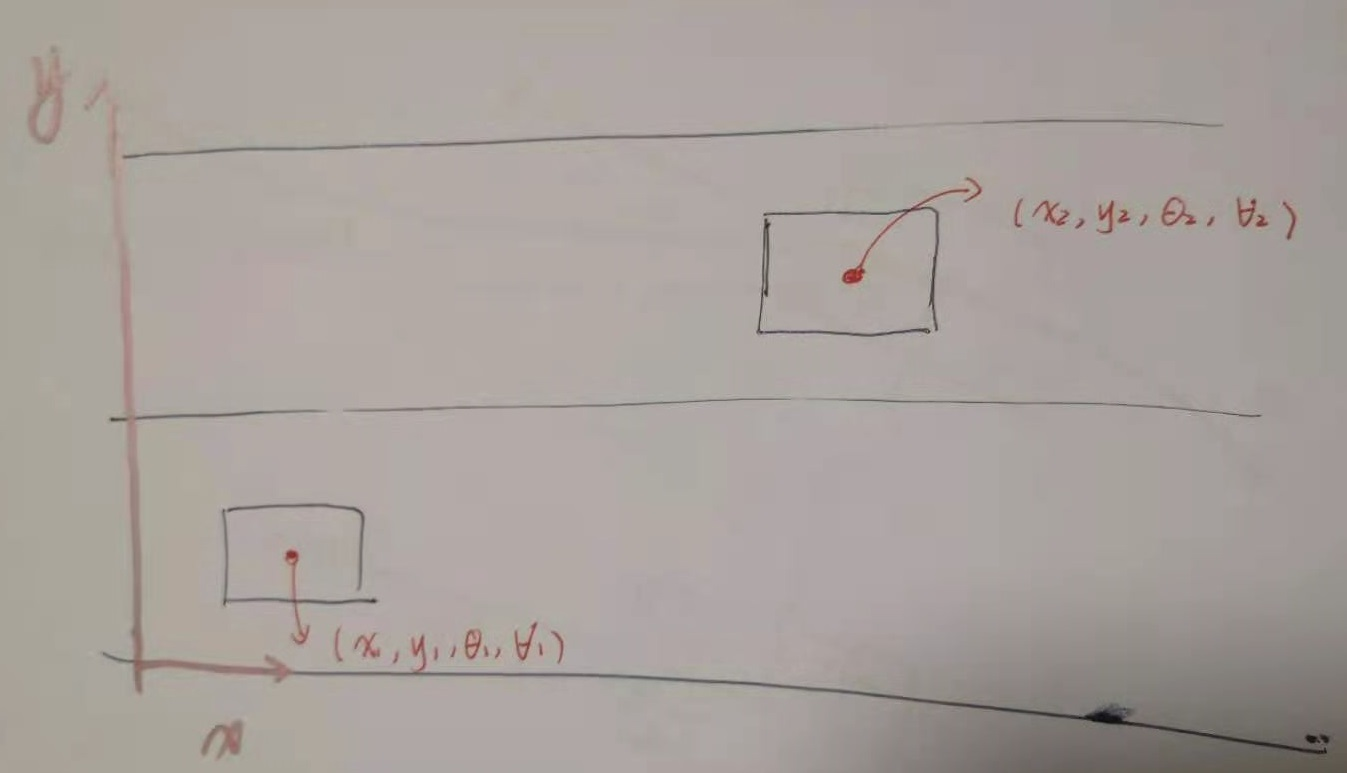
\includegraphics[width=5cm]{huandao.jpg}
\end{textblock}
  首选对整个系统建模(LQ微分博弈):
  $$
  \dot{x}(t) = A x(t) + B_1 u_1(t) + B_2 u_2(t), \quad x(0) = x_0,
  $$
  对于player 1(智能体,这里假设2个),对应的二次型性能函数为
  $$
  J_1(u_1,u_2) = \int_{0}^{T} \{ x^T(t) Q_1 x(t) + u^T_1(t) R_{11} u_1(t) + u^T_2(t) R_{12} u_2(t)  \} dt + x^T(T) Q_{1T} x(T),
  $$
  对player 2
  $$
  J_2(u_1,u_2) = \int_{0}^{T} \{ x^T(t) Q_2 x(t) + u^T_1(t) R_{21} u_1(t) + u^T_2(t) R_{22} u_2(t)  \} dt + x^T(T) Q_{2T} x(T),
  $$
  所有的矩阵都是对称矩阵,并且$R_{ii}$必须是正定矩阵.为了方便记号,记$S_i=B_i R^{-1}_{ii} B^T_i$
\end{frame}

\begin{frame}
\frametitle{LQ-Game}
\begin{itemize}
\item 定理


  定义矩阵
  $$
  M \coloneqq \begin{bmatrix}
  A &  -S_1 & -S_2 \\
 -Q_1 & -A^T & 0\\
 -Q_2 & 0 & -A^T
\end{bmatrix}
  $$
  假设两个Riccati微分方程
  $$
  \dot{K}_i(t) = - A^T K_i(t) A + K_i (t) S_i K_i(t) - Q_i, \, K_i(T) = Q_{iT}, \quad i=1,2
  $$
  有解且为对称阵$K_i(.)$.那么当
  $$
  H(T) \coloneqq \begin{bmatrix} I & 0 & 0 \end{bmatrix} e^{- M T} \begin{bmatrix} I \\ Q_{1T} \\ Q_{2T} \end{bmatrix}
  $$
  可逆时候,这个LQ微分博弈就有唯一的一个open-loop纳什均衡解(for every initial state $x_0$).这个解和对应的状态轨迹可以通过求解如下边值问题
  $$
  \dot{y}(t) = M y(t), \qquad P y(0) + Q y(T) = \begin{bmatrix} x^T_0 & 0 & 0 \end{bmatrix}^T
  $$

\end{itemize}
\end{frame}

\begin{frame}
\frametitle{LQ-Game}
\begin{itemize}
\item
  其中$y(t) = \begin{bmatrix} y^T_0(t) & y^T_1(t) & y^T_2(t) \end{bmatrix}^T, \, y_0 \in \mathbb{R}^n, \, y_i \in \mathbb{R}^{m_i}, i=1,2$, 均衡轨迹和控制率为
  $$
  x(t) = y_0(t), \qquad u_i(t) = - R^{-1}_{ii} B^T_i y_i(t), \quad i=1,2
  $$

  \item 证明(部分)

  假设$(u^*_1(.), u^*_2(.))$是纳什均衡,根据PMP原理, Hamiltonian是
  $$
  H_i = (x^T Q_i x + u^T_1 R_{i1} u_1 + u^T_2 R_{i2} u_2) + \psi^T_i (Ax + B_1 u_1 + B_2 u_2)
  $$
  最小化哈密度量得到
  \begin{align*}
    \begin{split}
      u^*_1 (t) = - R^{-1}_{11} B^T_1 \psi_1 (t), \\
      u^*_2 (t) = - R^{-1}_{22} B^T_2 \psi_2 (t),
    \end{split}
  \end{align*}
  其中
    \begin{align*}
    \begin{split}
    \dot{\psi}_{1}(t) &=-Q_{1} x(t)-A^{T} \psi_{1}(t), \text { with } \psi_{1}(T)=Q_{1 T} x(T) \\
    \dot{\psi}_{2}(t) &=-Q_{2} x(t)-A^{T} \psi_{2}(t), \text { with } \psi_{2}(T)=Q_{2 T} x(T) \\
    \dot{x}(t) &= A x(t) - S_1 \psi_1 (t) - S_2 \psi_2 (t)
    \end{split}
  \end{align*}
\end{itemize}
\end{frame}

\begin{frame}
\frametitle{LQ-Game}
\begin{itemize}
\item 证明(部分)

整理下动态系统为
$$
\frac{d}{d t}\left[\begin{array}{c}
x(t) \\
\psi_{1}(t) \\
\psi_{2}(t)
\end{array}\right]=M\left[\begin{array}{c}
x(t) \\
\psi_{1}(t) \\
\psi_{2}(t)
\end{array}\right]
$$
满足$x(0)=x_0$和$\psi_i(T)-Q_{iT}(T)=0$.设$y(t)=[x^T(t), \psi^T_1(t), \psi^T_2(t) ]^T$,则对于每一个$x_0$,这个问题变为linear two-point boundary value问题
$$
\dot{y}(t) = M y(t), \qquad \text{with} \, P y(0) + Q y(T) = [x^T_0, 0, 0]^T
$$.

\item 整理-简化

好比我们之前在单智能体中LQR中关于控制率做的那一套,首先假设$\psi_1 = P_1 x, \psi_2 = P_2 x$首先整理下现在的系统方程
\begin{align*}
  \begin{split}
     P_1 \dot{x} & = (-Q_1 - A^T P_1 - \dot{P}_1 ) x \\
     P_2 \dot{x} & = (-Q_2 - A^T P_2 - \dot{P}_2 ) x \\
     \dot{x} & = (A  - B_1 R^{-1}_{11} B^T_1 P_1  - B_2 R^{-1}_{22} B^T_2 P_2 )x
  \end{split}
\end{align*}
\end{itemize}
\end{frame}


\begin{frame}
\frametitle{LQ-Game}
\begin{itemize}
\item 整理-简化

得到Riccati 微分方程
\begin{align*}
  \begin{split}
     \dot{P}_1 & =   P_1 B_1 R^{-1}_{11} B^T_1 P_1  + P_1 B_2 R^{-1}_{22} B^T_2 P_2  - Q_1 - A^T P_1 - P_1 A \\
     & = P_1 S_1 P_1 + P_1 S_1 P_2 - Q_1 - A^T P_1 - P_1 A\\
     \dot{P}_2 & = P_2 B_1 R^{-1}_{11} B^T_1 P_1  + P_2 B_2 R^{-1}_{22} B^T_2 P_2  - Q_2 - A^T P_2 - P_2 A \\
     & = P_2 S_1 P_1 + P_2 S_1 P_2 - Q_2 - A^T P_2 - P_2 A
  \end{split}
\end{align*}
如果再假设$P_i$是恒定的值,那么可得到耦合Riccati代数方程
\begin{align*}
  \begin{split}
     0 & =  P_1 S_1 P_1 + P_1 S_1 P_2 - Q_1 - A^T P_1 - P_1 A\\
     0 & = P_2 S_1 P_1 + P_2 S_1 P_2 - Q_2 - A^T P_2 - P_2 A
  \end{split}
\end{align*}
我们设
$$
Q:=\left[\begin{array}{l}
Q_{1} \\
Q_{2}
\end{array}\right] ; \quad A_{2}:=\left[\begin{array}{ll}
A & 0 \\
0 & A
\end{array}\right] ; \quad A_{1}:=A ; \quad S:=\left[\begin{array}{ll}
S_{1} & S_{2}
\end{array}\right] \text { and } X:=\left[\begin{array}{l}
P_{1} \\
P_{2}
\end{array}\right]
$$
那么上面的代数方程可以写成
$$
Q + A^T_2 X + X A_1 - XSX = 0.
$$
\end{itemize}
\end{frame}

\section{算法设计}
\begin{frame}
\frametitle{iLQR-Game}

\begin{algorithm}[H]
\caption{Iterative LQ Games}%算法名字
\LinesNumbered %要求显示行号
\KwIn{初始状态$x_0$,初始控制策略$\{ \pi^0 \}_{i \in N}$}%输入参数
\KwOut{收敛的控制策略$\{ \pi^* \}_{i \in N}$}%输出
% some description\; %\;用于换行
\For{$k=1,2,\cdots$}{
    通过控制策略$\pi^k$得到状态轨迹 $\xi^k$ \;
    线性化轨迹得到 $A(t),B(t)$ \;
    二次化性能函数得到 $l_i,Q_i, R_{ij} $ \;
    求解LQ博弈得到下一步的控制策略 $\pi^{k+1}$ \;
  only if\;
  \If{收敛}{
    返回  $\pi^{k+1}$ \;
  }
    返回第一步 \;
}

\end{algorithm}

\end{frame}


\begin{frame}
\frametitle{iLQR-Game}
\begin{itemize}
  \item 更新的步长,要保证性能一直在优化的话步长不可以太大
  $$
  (1-\alpha)(\text{cost})+\alpha(\| x_t - x^k \|^2 + \| u_t - u^k \|^2)
  $$.
  \item 而且这里不可以通过线搜索来找到最优步长,因为各个智能体之间的性能函数可能冲突.
  \item 并没有任何理论保证可以从任意初始状态收敛.
  \item 大多数情况下收敛到局部最优解.
  \item 算法复杂度也不能保证,每一个LQ博弈的复杂度是$O(N^3 n^3)$,但是收敛需要的数量是不确定的(理论上).
  \item 论文里说避障问题小于$50ms$.
  \item 不能很好的保证约束得到满足.
  \item 论文视频,伯克利的Hybrid Systems Lab \url{https://www.youtube.com/watch?v=KPEPk-QrkQ8&ab_channel=BerkeleyHybridSystemsLab}
\end{itemize}
\end{frame}

\begin{frame}
\frametitle{ALM-Game:ALM 介绍和推导}
  考虑一个线性约束的优化问题
  $$
  \min \, f(x) \quad s.t. \quad Ax=b
  $$
  KKT条件是
  $$
  \nabla f(x^*)=- A^T \lambda^*, \quad A x^* = b.
  $$
  定义拉格朗日函数为
  $$
  \mathcal{L}(x, \lambda) = f(x) + \lambda^T (Ax-b)
  $$
  那么KKT条件就是
  $$
  \nabla \mathcal{L}(x^*, \lambda^*) =
  \begin{bmatrix}
    \nabla_x \mathcal{L}(x^*, \lambda^*) \\
    \nabla_{\lambda} \mathcal{L}(x^*, \lambda^*)
  \end{bmatrix} = 0
  $$
  定义增广拉格朗日函数为
  $$
  \mathcal{L}(x,\lambda;\rho) = \underbrace{f(x)+ \lambda^T (Ax-b)}_{\text{Lagrangian}} + \underbrace{\frac{\rho}{2} \| Ax-b \|^2_2}_{\text{"augmentation"}}
  $$
  那么基本的ALM更新方法是
  \begin{align*}
    \begin{split}
       x_k & = \mathop{\arg\min}_{x} \mathcal{L} (x, \lambda_{k-1}; \rho) \\
       \lambda_k   & = \lambda_{k-1} + \rho (A x_k -b)
    \end{split}
  \end{align*}
\end{frame}

\begin{frame}
\frametitle{ALM推导}
原问题可以写成
$$
\min_x \max_{\lambda} f(x) + \lambda^T (Ax-b)
$$
这个问题是和原问题是等价的,但是求解$\max$非常不光滑,我们通过"proximal point"光滑它,同时惩罚这个$\lambda$偏离我们对他的先验$\bar{\lambda}$,那么
$$
\min_x \big \{
\max_{\lambda} f(x) + \lambda^T (Ax-b) - \frac{1}{2 \rho} \| \lambda - \bar{\lambda} \|^2
\big \}
$$
这样最大化$\lambda$就是极为简单的一件事情了
$$
\lambda = \bar{\lambda} + \rho (Ax-b)
$$
再把这个结果带回去得到
$$
\min_x f(x) + \bar{\lambda} (Ax-b) + \frac{\rho}{2}
\| Ax -b \|^2 = \mathcal{L}(x, \bar{\lambda}; \rho)
$$
这样我们总结增广拉格朗日算法如下
\begin{enumerate}
  \item 最小化$\min_x \mathcal{L}(x, \bar{\lambda}; \rho)$得到新的$x$.
  \item 通过新得到的$x$来更新$\lambda = \bar{\lambda}+ \rho(Ax-b)$.
  \item 返回第一步直到收敛.
\end{enumerate}
\end{frame}

\begin{frame}
\frametitle{ALM推导}
把问题推广到线性不等式约束
$$
\min f(x) \quad s.t. \quad Ax \ge b.
$$
用相同的方法转化下
$$
\min_x \max_{\lambda \ge 0} f(x) - \lambda^T (Ax-b).
$$
在寻找最优$\lambda$需要一个分类操作
$$
\max (\bar{\lambda} + \rho (Ax-b), 0)
$$
最后,对于非线性约束$c(x)=0$或者$c(x) \ge 0 $可使用相同方法推导。
\end{frame}

\begin{frame}
\frametitle{ALM-GAME问题描述}
考虑如下系统
$$
x_{k+1} = f (x_k, u^1_k, \cdots, u^M_k ) = f( x_k, u_k )
$$
运动学约束为
$$
D(X,U^1,\cdots,U^M) = D(X,U) = 0
$$
还有一些约束是和其他玩家状态有关,我们表示这样的约束为
$$
C(X,U) \le 0
$$
对于每一个玩家,他做的事情可以写成这样
\begin{align*}
\begin{split}
   \min_{X, U^v} \quad & J^v (X, U^v) \\
    s.t. \qquad & D(X, U) = 0, \\
    & C(X, U) \le 0.
\end{split}
\end{align*}
我们把这样的约束问题写成ALM形式
$$
L^v(X,U) = J^v + {u^v}^T D + \lambda^T C + \frac{1}{2} C^T I_p C
$$
根据局部最优性可得
$$
\nabla_{X,U^v} L^v(X,U,u^v) = G^v(X,U,u^v)=0
$$
\end{frame}

\begin{frame}
\frametitle{ALM-GAME问题描述}
我们把所有玩家的最优性方程都联立起来,就得到了这样的方程
\begin{align*}
\begin{split}
   \min_{X, U^v} \quad & 0 \\
    s.t. \qquad & G^v(X,U,u^v)=0, \quad \forall v \in \{ 1,\cdots,M \} \\
    & D(X, U) = 0.
\end{split}
\end{align*}
我们把所有梯度联立为一个变量$G(X,U,u) = [ (G^1)^T,\cdots,(G^M)^T,D^T ]^T$,其中$u=[ (u^1)^T,\cdots, (u^M)^T ]^T$ 这样我们对$G$做梯度即为
$$
H = \nabla_{X,U,u} G = \nabla_y G
$$
通过牛顿法来确定方向
$$
\delta y = - H^{-1} G
$$
然后步长就通过Backtracking line-search来确定.
\end{frame}

\begin{frame}
\frametitle{ALM-GAME算法}
\begin{algorithm}[H]
\caption{ALGAMES solver}%算法名字
\LinesNumbered %要求显示行号
\KwIn{初始参数$\rho_0,\lambda, u^v,X^(0),U(0)$}%输入参数
\KwOut{收敛的$y$}%输出
% some description\; %\;用于换行
\While{不收敛}{
    $y \leftarrow$ NEWTON's METHOD$(y)$ \;
    $\lambda \leftarrow$ DUALASCENT$(y,\lambda,\rho)$ \;
    $\rho \leftarrow$ INCREASINGSCHEDUAL$(\rho)$ \;
}

返回 $y$ \;

\end{algorithm}

\begin{itemize}
  \item 这里的$\lambda$更新规则是
  $$
  \lambda_k \leftarrow \left \{ 
  \begin{array}{ll}
    \max (0, \lambda_k + \rho_k C_k(C,U) ) & k \leq n_{ci}\\
    \lambda_k + \rho_k C_k(X,U) & n_{ci} \leq k \leq n_{ci} + n_{ce}
  \end{array} \right.
  $$
  \item $\rho$的更新规则是
  $$
  \rho_k \leftarrow  \gamma \rho_k
  $$
\end{itemize}

\end{frame}

\begin{frame}
\frametitle{Controllability of Nash Equilibrium in Game-Based Control Systems}
系统建模
$$
\left\{\begin{aligned}
\dot{x}(t) &=f\left(t, x(t), x_{1}(t), \ldots, x_{L}(t), u_{1}(t), \ldots, u_{L}(t), u(t)\right) \\
\dot{x}_{i}(t) &=f_{i}\left(t, x(t), x_{1}(t), \ldots, x_{L}(t), u_{1}(t), \ldots, u_{L}(t), u(t)\right) \\
x(0) &=x_{0}, x_{i}(0)=x_{i, 0}, i=1,2, \ldots, L, t \in[0, T]
\end{aligned}\right.
$$

每个玩家的性能指标
$$
\begin{array}{l}
J_{i}\left(u_{1}(\cdot), u_{2}(\cdot), \ldots, u_{L}(\cdot)\right) \\
\quad=K_{i}\left(x^{F}(T)\right)+\int_{0}^{T} L_{i}\left(X(\cdot), u_{1}(\cdot), u_{2}(\cdot), \ldots, u_{L}(\cdot)\right) d t
\end{array}
$$
开环纳什均衡
$$
\left\{\begin{aligned}
\dot{x}^{*}(t) &=f\left(t, X^{*}(t), u_{1}^{*}(t), \ldots, u_{L}^{*}(t), u(t)\right) \\
\dot{x}_{i}(t) &=f_{i}\left(t, X^{*}(t), u_{1}^{*}(t), \ldots, u_{L}^{*}(t), u(t)\right) \\
x^{*}(0) &=x_{0}, x_{i}(0)=x_{i, 0}, i=1,2, \ldots, L
\end{aligned}\right.
$$
\end{frame}

\begin{frame}
\frametitle{GBCS}
\begin{definition}[可控性]
If for any given
initial states $x(0) = x_0 \in  \mathbb{R}^n$ , $x_i (0) = x_i(0) \in  \mathbb{R}^{n i} , i = 1, 2, \cdots , L$,
and any terminal macro state $x(T) = x_T \in  \mathbb{R}^n$ , there is a strategy
$u(t)(t \in [0, T ])$ of the regulator, under which the Nash equilibrium
exists and is unique, and the solution $x^* (t)$ satisfies $x^*(T )
= xT$ .
\end{definition}
考虑线性二次型系统
$$
\left\{\begin{aligned}
\dot{x}(t)=& A(t) x(t)+\sum_{i=1}^{L} A_{i}(t) x_{i}(t)+\sum_{i=1}^{L} D_{i}(t) u_{i}(t) 
+B(t) u(t) \\
\dot{x}_{i}(t)=& E_{i}(t) x(t)+\sum_{j=1}^{L} F_{i j}(t) x_{i}(t)+\sum_{j=1}^{L} B_{i j}(t) u_{j}(t) 
+B_{i}(t) u(t) \\
x(0)=& x_{0}, x_{i}(0)=x_{i, 0}(i=1,2, \ldots, L)
\end{aligned}\right.
$$
每个玩家性能指标
$$
\begin{array}{l}
J_{i}\left(u_{1}(\cdot), u_{2}(\cdot), \ldots, u_{L}(\cdot)\right)=\frac{1}{2} x^{F}(T)^{T} Q_{i T} x^{F}(T) \\
\quad+\frac{1}{2} \int_{0}^{T}\left[X^{T}(t) Q_{i}(t) X(t)+u_{i}^{T}(t) R_{i}(t) u_{i}(t)\right] d t
\end{array}
$$
\end{frame}

\begin{frame}
\frametitle{GBCS}
假设下面的Riccati微分方程有解$K_j$
$$
\left\{\begin{aligned}
\dot{K}_{j}(t) &=-\widetilde{A}^{T} K_{j}-K_{j} \widetilde{A}-Q_{j}+K_{j} \widetilde{S}_{j} K_{j} \\
K_{j}(T) &=\widetilde{Q}_{j T}
\end{aligned}\right.
$$
定义转移矩阵$\Phi(t)$和可控的格拉姆矩阵$W$为
$$
\left\{\begin{aligned}
\frac{d \Phi(t)}{d t} &=-\Phi(t) \bar{A}(t) \\
\Phi(0) &=I_{(L+1) N}
\end{aligned}\right.
\qquad 
W(T)=\int_{0}^{T} \Phi(t) \bar{B}(t) \bar{B}^{T}(t) \Phi^{T}(t) d t
$$

\begin{theorem}
  GBCS系统可控仅当下面矩阵满秩的时候
  $$
  \left[\left[\begin{array}{c}
    0_{N \times(L N)} \\
    I_{N L}
    \end{array}\right], \Phi(T) Q_{T}\left[\begin{array}{c}
    0_{n \times(N-n)} \\
    I_{N-n}
    \end{array}\right], W(T)\right]
  $$
\end{theorem}
\end{frame}

\section{仿真实验}
\begin{frame}



\end{frame}

\thispagestyle{empty} 
\begin{frame}{}
  \centering \Huge
  \emph{Thank You}
\end{frame}
\end{document}
%%% Local Variables:
%%% mode: latex
%%% TeX-master: t
%%% TeX-engine: xetex
%%% End:
